% Position Calculation


\chapter{Position Calculation} % Main chapter title

\label{PositionCalculation}

%----------------------------------------------------------------------------------------

This chapter covers the position calculation subsystem, which takes the ranges from the rangefinding subsystem and calculates their positions. It also covers how the subsystem is integrated into the augmented reality subsystem. The position subsystem is not a separate piece of hardware. Rather, it is just a very complex mathematical function. An example of possible positions calculated from range data is shown in Figure~\ref{fig:FrameOfReference}.

The topics covered in this chapter are:
\begin{enumerate}
	\item The infinite possible positions able to be calculated from a set of ranges.
	\item A high-level example of calculating positions with basic trigonometry in 2D.
	\item How this is extended to 3D.
	\item The protocol used by the Arduinos to communicate with the cell phones of the users and transfer the ranging data.
\end{enumerate}

\section{Frame of Reference}
\label{FrameOfReference}
\begin{figure}
	\centering
	\tikzstyle{vertex}=[circle, draw]
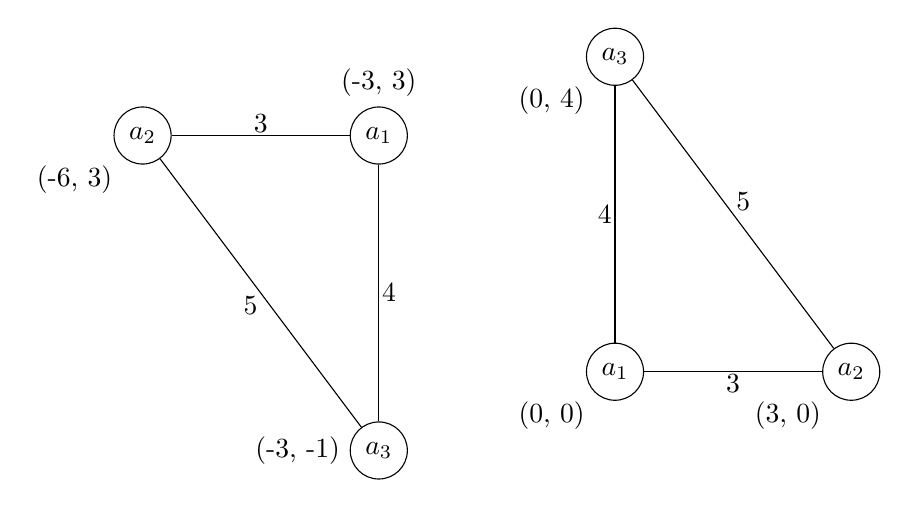
\begin{tikzpicture}[transform shape]
\node[vertex,label=below left:{(0, 0)}](a1) at (0, 0) {$ a_1 $};
\node[vertex,label=below left:{(3, 0)}](a2) at (3, 0) {$ a_2 $};
\node[vertex,label=below left:{(0, 4)}](a3) at (0, 4) {$ a_3 $};

\begin{scope}[every path/.style={-}, every node/.style={inner sep=1pt}]
       \draw (a1) -- node [anchor=north] {$3$} (a2);
       \draw (a2) -- node [anchor=south west] {$5$} (a3);
       \draw (a1) -- node [anchor=east] {$4$} (a3);
\end{scope} 

\node[vertex,label=above:{(-3, 3)}](a4) at (-3, 3) {$ a_1 $};
\node[vertex,label=below left:{(-6, 3)}](a5) at (-6, 3) {$ a_2 $};
\node[vertex,label=left:{(-3, -1)}](a6) at (-3, -1) {$ a_3 $};

\begin{scope}[every path/.style={-}, every node/.style={inner sep=1pt}]
       \draw (a4) -- node [anchor=south] {$3$} (a5);
       \draw (a5) -- node [anchor=north east] {$5$} (a6);
       \draw (a4) -- node [anchor=west] {$4$} (a6);
\end{scope} 
\end{tikzpicture}
	\decoRule
	\caption{Two example networks with different positions reporting the same ranges.}
	\label{fig:FrameOfReference}
\end{figure}

One of the most important aspects to understanding the position of an object in space is knowing what it is \emph{relative} to. If a point $p = (x, y, z) = (1, 2, 3)$, this is not useful unless it is known where, say, $(0, 0, 0)$ is and what directions the various axes point in.

The rangefinding subsystem determines the ranges between various devices. With these ranges, we can use trigonometry and determine positions in 3D space. However, it is impossible to place the positions in such a way that they correspond to the real world with only the range information. There are many different possible sets of positions which will result in the same rangefinding data. Figure~\ref{fig:FrameOfReference} shows two possible sets of positions that will result in the rangefinding system reporting the same ranges.

In order to cut down on the infinite possible solutions to finding positions given only range data, this subsystem must arbitrarily create its own system of coordinates. The positions calculated by this subsystem must be further transformed so as to correspond to the real world. This transformation is not covered in this chapter, and instead is dealt with in Section~\ref{Calibration}.

\section{High-Level Example in 2D}

\begin{figure}
	\centering
	\tikzstyle{vertex}=[circle, draw]
\begin{tikzpicture}[transform shape]
\node[vertex](a0) at (0, 0) {$ a_0 $};
\node[vertex](a1) at (6, 0) {$ a_1 $};
\node[vertex](a2) at (1.5, 4.3) {$ a_2 $};


\begin{scope}[every path/.style={-}, every node/.style={inner sep=1pt}]
       \draw (a0) -- node[align=center, anchor=north] {$d_{01}$} (a1);
       \draw (a0) -- node[align=center, anchor=south east] {$d_{02}$} (a2);
       \draw (a1) -- node[align=center, anchor=south west] {$d_{12}$} (a2);
\end{scope} 
\end{tikzpicture}
	\decoRule
	\caption{A network with 3 anchors $a_i$ and the reported distances between them.}
	\label{fig:PositionCalculationNetwork}
\end{figure}

As 3D position calculation is much more complex, position calculation is done in 2D will be explained first. We start with the distances between three anchors, $a_{0}$, $ a_{1}$  and $a_{2}$. The distance between anchor $i$ and anchor $j$ is $d_{ij}$. 

In order to assign positions in 2D space to them that keep them the same ranges from each other, we start by setting $a_{0}$ arbitrarily to be at the origin. Next, we arbitrarily declare $a_{1}$ to be on the x-axis, which puts it at the position $(0, d_{01})$. With these two positions, we can calculate the angle $\Theta$ between the x-axis and the vector from $a_0$ to $a_2$ with the cosine law:

\[ \Theta = \cos ^{-1}\Big(\frac{d_{01}^2 + d_{02}^2 - d_{12}^2 }{2 d_{01} d_{02}}\Big)\]

With $\Theta$, we can calculate x and y coordinates of $a_2$:

\[ x = cos(\Theta) d_{12} \]
\[ y = sin(\Theta) d_{12} \]

\section{Extending This to 3D}
Extending the subsystem to three dimensions does not really change the calculation all that much except that we now need four anchors to get a reliable position in three dimensions. We have our four anchors: $a_{0}$, $a_{1}$ , $a_{2}$ and $a_{3}$, we arbitrarily set one as the origin $a_{0}$(0, 0, 0) and we now make a horizontal line to another anchor say $a_{1}$ and since we know the distance between these two anchors we can get the position to be $a_{1}$(0, $d_{01}$, 0), where $d_{01}$ is the distance between $a_{0}$ and $a_{1}$. We can now form a triangle with the third anchor and use cosine law to determine the position and we arbitrarily set the z value to 0.
\\
We now have the coordinates for the third anchor, but we do not know the correct orientation in the z axis, it could be either positive or negative. This is where the fourth anchor comes in, we use the anchor to create a temporary point using the same method we use above.
\\
\[ \Theta = \cos ^{ - 1}\Big(\frac{d_{01}^2 + d_{03}^2 - d_{13}^2 }{2 d_{01} d_{03}}\Big)\]
\\
\[ x_{temp} = cos(\Theta) d_{13} \]
\[ y_{temp} = sin(\Theta) d_{13} \]
\[ z_{temp} = 0 \]
\\
We will rotate around the x-axis by keeping the x value constant and taking the y distance and z distance to be a circle of radius of $y_{temp}$.We calculate the distance between the x value of the temporary point and the x value of anchor 2, we denote this value $\Delta x$.
\\
\[ \Delta x = x_{temp} - x_{2} \]
\\
Now that we have $\Delta x$ we can now calculate the position of our fourth anchor using cosine law.
\\
\[\Theta = \cos ^{ - 1}\Big(\frac {\Delta x^2 - d_{23}^2 + y_{2}^2 + y_{temp}^2}{2 y_{2} y_{temp}}\Big)\]
\\
\[ x_{3} = x_{temp} \]
\[ y_{3} = cos(\Theta) y_{temp} \]
\[ z_{3} = sin(\Theta) y_{temp} \]

\section{Integrating Rangefinding and Position Calculation}
The position calculation code runs on the cellphone. In order to calculate positions, ranges must be transferred to the cellphone from the Arduino Pro Mini. 

The Arduino's processor can communicate serially via UART TTL. Most cellphones do not have the ability to communicate serially, but Future Technology Devices International (FTDI) manufactures a USB cable that interfaces between the serial output of the Arduino and the micro USB port of a cellphone. With this cable connecting an Arduino and a cellphone, the cellphone can provide power to the Arduino and send and receive data to it.

The project uses the Android \code{D2xx} library, provided by FTDI, to communicate with the Arduino while running an Android app. It allows the easy sending and receiving of bytes. 

\section{Protocol}
There are a number of design considerations when dealing with the communications between the cellphone and the Arduino:
\begin{enumerate}
	\item The stream of data may begin in the middle of a message, as the buffer storing the serial data sent from the Arduino has only a limited capacity. If a cellphone were connected to an anchor that had already been running for some time, it is quite likely that the buffer would have overflowed. So, the protocol must include a way to determine the start of a message.
	\item The protocol should be human readable for easy debugging.
\end{enumerate}

With this in mind, a simple protocol was developed. Lines of text, delineated by newline characters, are sent. If the Arduino is reporting the range between two devices, it sends a line with the format:

\begin{center}
\code{!range <from ID> <to ID> <range in meters>}
\end{center}

If the cellphone reads a line which does not start with ``!r'', the line is assumed to either have started in the middle of a ranging information line, or else debug data has been sent. Either way, the line is discarded and the system waits to read a new line.

An example of the output from the Arduino is:

\code{\\
DW1000 initialized ... \\
Committed configuration ... \\
New device found. ID: 1 \\
Transmission received from tag 1 with transmission count 1 \\
!range 1 2 0.00 \\
Transmission received from tag 1 with transmission count 3 \\
!range 2 1 3.26 \\
!range 1 2 91659.28 \\
Transmission received from tag 1 with transmission count 5 \\
!range 2 1 3.48 \\
!range 1 2 3.38 \\
Transmission received from tag 1 with transmission count 7 \\
!range 2 1 3.37 \\
!range 1 2 3.42 \\
}

Note the briefly extremely large range while the timestamps settle.

Parsing is done on the cellphone with the \code{java.util.Scanner} class. The parsing code can be found in (INSERT THIS LATER).

\section{Summary}
This chapter covered the issues with the infinite possible positions that can be calculated from a set of ranges between nodes, the math behind calculating positions in 3D given ranges, and how the cellphones and Arduinos are interfaced.